% Charlotte Geiger - Manuel Lippert - Leonard Schatt
% Physikalisches Praktikum

% Teilauswertung 2

\section{Nutation}

\begin{itemize}
    \item Für jede Frequenz $\frac{w_n}{w_3} = \frac{J_3-J_1}{J_1}$ $\Rightarrow$ Tabelle
    \item $\frac{w_n}{w_3}$ gegen $w_3$ $\Rightarrow$ Zeichnung
\end{itemize}

Die Nutation ist eine zus\"atzliche Komponente zur Präzession. Bei genauer Beobachtung des Kreisels kann man neben der Präzessionsbewegung erkennen, dass die Kreiselachse nicht komplett ruhig um die Senkrechte läuft, sondern viel mehr kleine Rotationen auf der Bahn der Präzession vollführt. Das ist das Phänomen der Nutation.\\
Um diese Nutation des Kreisels zu untersuchen, bestimmt man die Nutationsfrequenz des momentfreien Kreisels als Funktion von $\omega_3$. Damit es gut darzustellen und auszuwerten ist, betrachtet man $w_3$ im Bezug zu $\frac{w_n}{w_3}$. \\
Um die Frequenz in die Winkelgeschwindigkeit umzurechnen, muss man die Frequenz mit $2\pi$ multiplizieren $(w = f\cdot2\pi)$.\\
Der Fehler des Stroboskoplichts ist der Ablesefehler $s_a = 0,05 1/s$. %TODO #1 @Charlie318 
Auch bei der Zeitmessung muss der Fehler mitbetrachtet werden, dieser beläuft sich auf $s_a = 0,5s$.
\begin{gather}
    \omega_3 = f_3\cdot2\pi  \tab s_{\omega_3}=2\pi\cdot{s_{f_3}} \\[0.3mm]
    \omega_n = \frac{2\pi}{T_n} \\[0.3mm]
    \frac{\omega_n}{\omega_3} = \frac{1}{T_nf_3} 
    \tab s_{\frac{\omega_n}{\omega_3}} = \sqrt{{(\frac{s_{T_n}}{T_n^2f_3})}^2+{(\frac{s_{f_3}}{T_nf_3^2})}^2} 
\end{gather} \\
Um das Verh\"altnis von $w_3$ im Bezug zu $\frac{w_n}{w_3}$ tabellarisch aufzutragen, muss man auf das Vorzeichen achten. Aus den Eulerschen Gleichungen f\"r den momentfreien, symmetrischen Kreisel wurde folgendes im Skript hergelitten:
\begin{align}
    \frac{\omega_n}{\omega_3} = \frac{J_3 - J_1}{J_1} = konstant
\end{align} \\
Da wir aber nur noch einen symmetrischen Kreisel mit $J_1 = J_2$ und $J_3<J_1$ betrachten, ist das konstante Verh\"altnis  negativ. Nun wird die Konstante durch den Mittelwert der berechneten Verh\"altnisse berechnet.
\begin{gather}   
    \overline{\Bigl(\frac{\omega_n}{\omega_3}\Bigr)} = \sum\nolimits_{i=1}^{12}\Bigl(\frac{\omega_n}{\omega_3}\cdot{\frac{1}{12}}\Bigr) \tab i: Anzahl der Werte\\
    s_{\overline{\frac{\omega_n}{\omega_3}} }= \frac{1}{12}\sqrt{\sum\nolimits_{i=1}^{12}{\Bigl(s_{\frac{\omega_n}{\omega_3}}\Bigr)}^2}=
\end{gather} \\
Somit folgt: 
\begin{equation}
    \frac{J_3-J_1}{J_3}= konstant
\end{equation}
Der hier berechnete Mittelwert ist das arithmetische Mittel beider Messreihen um seinen Fehler. Diese werden nun in das Diagramm eingef\"ugt und gegen die Drehfrequenz $\omega_3$ aufgetragen. 
%konntet ihr hier bitte die Tabelle (Nutation_in Auswertung_Kre) und den Plot (omega_v gegen omega_3) einfügen 
%TODO #4 @ManeLippert

% Table generated by Excel2LaTeX from sheet '6.2 Nutation'
\begin{table}[htbp]
    \centering
      \begin{tabular}{cccccccc}
      \rowcolor[rgb]{ .741,  .843,  .933} $f_3$ [Hz] & $s_{f_3}$ [Hz] & $t_{n_1}$ [s] & $t_{n_2}$ [s] & $t_n$ [s] & $s_{t_n}$ [s] & $T_n$ [s] & $s_{T_n}$ [s] \\
      10.0  & 0.05  & 62.69 & 59.96 & 61.33 & 0.01  & 6.27  & 0.001 \\
      10.5  & 0.05  & 58.84 & 59.50 & 59.17 & 0.01  & 5.88  & 0.001 \\
      11.0  & 0.05  & 56.94 & 59.69 & 58.32 & 0.01  & 5.69  & 0.001 \\
      12.0  & 0.05  & 51.53 & 51.13 & 51.33 & 0.01  & 5.15  & 0.001 \\
      13.0  & 0.05  & 49.63 & 48.87 & 49.25 & 0.01  & 4.96  & 0.001 \\
      14.0  & 0.05  & 44.75 & 45.56 & 45.16 & 0.01  & 4.48  & 0.001 \\
      15.0  & 0.05  & 40.78 & 40.53 & 40.66 & 0.01  & 4.08  & 0.001 \\
      16.0  & 0.05  & 37.47 & 38.28 & 37.88 & 0.01  & 3.75  & 0.001 \\
      17.0  & 0.05  & 35.71 & 36.31 & 36.01 & 0.01  & 3.57  & 0.001 \\
      18.0  & 0.05  & 34.25 & 34.65 & 34.45 & 0.01  & 3.43  & 0.001 \\
      19.0  & 0.05  & 32.85 & 33.06 & 32.96 & 0.01  & 3.29  & 0.001 \\
      20.0  & 0.05  & 30.75 & 31.19 & 30.97 & 0.01  & 3.08  & 0.001 \\
      \end{tabular}%
    \label{tab:addlabels}%
    \caption{Add caption}
\end{table}%

% Table generated by Excel2LaTeX from sheet '6.2 Nutation'
\begin{table}[htbp]
    \centering
      \begin{tabular}{cccccc}
      \rowcolor[rgb]{ .741,  .843,  .933} $w_3$ [$\frac{1}{s}$] & $s_{w_3}$ [$\frac{1}{s}$] & $w_n$ [$\frac{1}{s}$] & $s_{w_n}$ [$\frac{1}{s}$] & $\frac{w_n}{w_3}$ & $s_\frac{w_n}{w_3}$  \\
      62.8  & 0.3   & 1.002 & 0.013 & 0.01595 & 0.00008 \\
      66.0  & 0.3   & 1.068 & 0.013 & 0.01619 & 0.00008 \\
      69.1  & 0.3   & 1.103 & 0.014 & 0.01597 & 0.00007 \\
      75.4  & 0.3   & 1.219 & 0.015 & 0.01617 & 0.00007 \\
      81.7  & 0.3   & 1.266 & 0.016 & 0.01550 & 0.00006 \\
      88.0  & 0.3   & 1.404 & 0.018 & 0.01596 & 0.00006 \\
      94.2  & 0.3   & 1.541 & 0.019 & 0.01635 & 0.00005 \\
      100.5 & 0.3   & 1.677 & 0.021 & 0.01668 & 0.00005 \\
      106.8 & 0.3   & 1.760 & 0.022 & 0.01647 & 0.00005 \\
      113.1 & 0.3   & 1.835 & 0.023 & 0.01622 & 0.00005 \\
      119.4 & 0.3   & 1.913 & 0.024 & 0.01602 & 0.00004 \\
      125.7 & 0.3   & 2.043 & 0.026 & 0.01626 & 0.00004 \\
      \end{tabular}%
    \label{tab:addlabel}%
    \caption{Add caption}
\end{table}%  

\begin{center}
    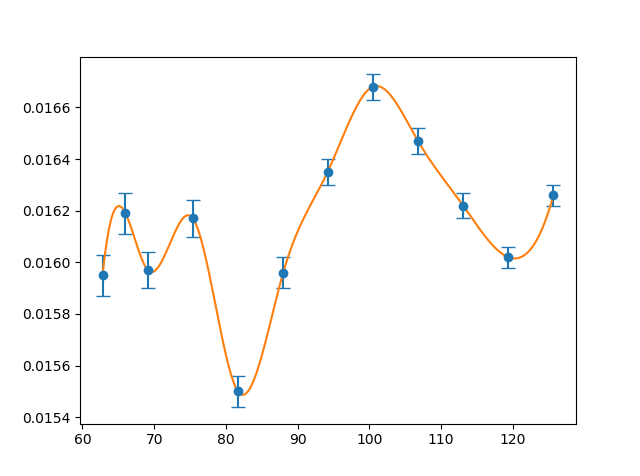
\includegraphics[scale=0.7]{6_2-Nutation_SplinePlot.png}
\end{center}
  